\documentclass[aps,twocolumn,floatfix,superscriptaddress,nofootinbib]{revtex4-2}

\usepackage{amsmath,amssymb,bm}
\usepackage{graphicx}
\usepackage{xcolor}
\usepackage{hyperref}

\hypersetup{
  colorlinks=true,
  linkcolor=blue,
  citecolor=blue,
  urlcolor=blue
}

\newcommand{\Tr}{\operatorname{Tr}}
\newcommand{\avg}[1]{\overline{#1}}
\newcommand{\Gtraj}{G_{\xi}}
\newcommand{\Gps}{G_{\rm ps}}
\newcommand{\Gbar}{\overline{G_{\xi}}}
\newcommand{\calL}{\mathcal{L}}
\newcommand{\calC}{\mathcal{C}}
\newcommand{\dd}{\mathrm{d}}

\begin{document}

\title{Trajectory-resolved adaptive preparation of a charge-fluctuating chiral critical ensemble}

\author{Asadullah Bhuiyan}
\affiliation{Department of Physics, Cornell University, Ithaca, New York 14853, USA}

\date{\today}

\begin{abstract}
This note summarizes the present numerical evidence that the finite-range class-A adaptive
fermion circuit prepares a charge-fluctuating, quasi-one-dimensional chiral critical ensemble
localized at a Chern-insulator domain wall.  The central distinction is ensemble-theoretic.
The physically meaningful ideal protocol is trajectory-resolved perfect correction: Born
measurement outcomes are sampled, ideal feedback is applied, and observables are averaged
over the resulting random Gaussian trajectories.  Post-selection, the deterministic Markov
channel, and its continuous-time Lindblad limit remove this randomness in inequivalent
ways and should be regarded as controls.  The existing data show robust logarithmic
entanglement scaling near the chiral-fermion value, purification toward a topological
domain-wall ensemble, persistent charge-sector fluctuations under perfect correction,
strong suppression of such fluctuations under post-selection, and modular-charge spreading
consistent with opposite chirality on opposite walls.  The evidence is coherent enough to
support the paper narrative, but not yet sufficient to close all finite-size and correlator
universality questions.
\end{abstract}

\maketitle

\section{Purpose and relation to the previous work}

Ref.~\cite{BhuiyanPanJian2026} developed the general framework: fermionic dynamics with
measurements can be classified by many-body evolution-operator and single-particle transfer
matrix symmetry classes, and class-A Gaussian adaptive circuits can prepare and stabilize
Chern-insulator states without post-selection.  It also identified dynamical domain-wall
modes and a separation between trajectory-resolved and trajectory-averaged transitions.

The present note is narrower and more diagnostic.  It asks whether the finite-range
class-A adaptive circuit, in a domain-wall geometry, prepares not merely a topological
bulk slab but a quasi-one-dimensional chiral critical state ensemble on the wall.  The
answer suggested by the current data is affirmative, provided that one keeps the ensemble
structure explicit.  Perfect correction is not equivalent to post-selection, and neither is
equivalent to evolving the averaged covariance matrix.  This difference is not a technical
detail: it is the mechanism behind the observed charge-fluctuating phenomenology.

\section{Four dynamical objects}

The top-layer Gaussian state in a trajectory is encoded by a covariance matrix $G_\xi$,
or equivalently by the one-body density matrix
\begin{equation}
  C_\xi = \frac{1+G_\xi}{2}.
\end{equation}
The measurement record $\xi$ labels the sequence of Born outcomes.  A nonlinear observable
$O$ defines at least three inequivalent quantities:
\begin{equation}
  \avg{O[\Gtraj(t)]}
  \neq O[\Gbar(t)]
  \neq O[\Gps(t)] .
  \label{eq:three_ensembles}
\end{equation}
Figure~\ref{fig:taxonomy} summarizes the taxonomy.

\begin{figure}[t]
  \centering
  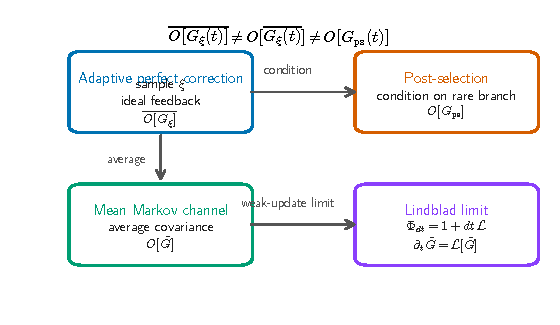
\includegraphics[width=\columnwidth]{figures/protocol_taxonomy.pdf}
  \caption{The four descriptions used in this note.  Perfect correction is the
  trajectory-resolved adaptive ensemble.  Post-selection is a fixed conditioned branch.
  The Markov channel evolves the mean covariance.  The Lindblad equation is the weak-update
  continuous-time limit of that mean channel.}
  \label{fig:taxonomy}
\end{figure}

\subsection{Adaptive perfect correction}

In the physical ideal protocol, measurement outcomes are sampled with their Born
probabilities.  Whenever an outcome disagrees with the target band occupation, ideal
feedback applies the corresponding correction.  In code language, a failed empty-band
condition triggers deterministic pump-out feedback, and a failed filled-band condition
triggers deterministic pump-in feedback.  The measurement outcome itself is still random.
The trajectory remains Gaussian, but the ensemble does not collapse to a single covariance.
The natural object is therefore
\begin{equation}
  \avg{O[\Gtraj]} = \sum_{\xi} p_\xi O[G_\xi],
\end{equation}
with $p_\xi$ determined dynamically by the Born rule.

\subsection{Post-selection}

Post-selection follows only the branch in which every measurement outcome is already the
desired one.  It computes $O[\Gps]$, where $\Gps$ is a conditioned covariance.  This is a
useful reference because it exposes what the adaptive circuit would do if measurement-record
randomness were removed rather than corrected.  The numerical driver correspondingly forces
the post-selected run to a single branch.  It is not a physical preparation protocol: the
selected branch has exponentially small weight in system size and time in generic monitored
dynamics.

\subsection{Mean Markov channel}

The deterministic routine \texttt{run\_markov\_channel} evolves a single covariance by the
Born-rule averaged local channel.  It gives a discrete map
\begin{equation}
  \Gbar_{n+1} = \Phi(\Gbar_n),
\end{equation}
and therefore computes $O[\Gbar]$.  This is distinct from $\avg{O[\Gtraj]}$ whenever
$O$ is nonlinear.  Entanglement entropies, entanglement contours, Chern markers built from
regularized spectra, and squared correlation functions all fall into this nonlinear class.
The existing correlation-profile comparison in Fig.~\ref{fig:mean_channel} makes the
distinction visible directly.

\subsection{Lindblad limit}

The continuous-time Lindbladian construction in Ref.~\cite{BhuiyanPanJian2026} and in the
related internal Lindblad note is the weak-success-probability limit of the mean channel.
For a local elementary channel $\Phi_{dt}$,
\begin{equation}
  \Phi_{dt} = 1 + dt\,\calL + O(dt^2),
  \qquad
  \partial_t \Gbar = \calL[\Gbar].
  \label{eq:lindblad_limit}
\end{equation}
This limit is analytically valuable: it identifies the jump-process structure of the
trajectory-averaged preparation and explains convergence toward the Chern-insulator
covariance.  Discrete data at update probability $p=1$ are Markov-channel data, not by
themselves a controlled continuous-time extrapolation.  The Lindblad limit should therefore
not be interpreted as a substitute for trajectory-resolved adaptive dynamics.

\section{Target domain-wall critical theory}

The target fixed point is the interface between a class-A Chern slab and a trivial
exterior.  In the ideal continuum description the wall carries a chiral complex fermion
with central charge $c=1$.  For an interval of length $\ell$ on a periodic edge of length
$L_y$, the entanglement contribution scales as
\begin{equation}
  S(\ell) =
  \frac{c}{3}
  \log\left[
    \frac{L_y}{\pi a}
    \sin\left(\frac{\pi \ell}{L_y}\right)
  \right]
  + s_0
  \quad (c=1),
  \label{eq:edge_entropy}
\end{equation}
when the full transverse support of both domain walls is included.  The squared equal-time
fermion correlation along the wall is expected to decay as
\begin{equation}
  |C(y)-C(0)|^2 \sim
  \left[
    \frac{L_y}{\pi}
    \sin\left(\frac{\pi |y|}{L_y}\right)
  \right]^{-2}.
  \label{eq:corr_target}
\end{equation}
The exact flattened-Hamiltonian domain-wall benchmark supplies the calibration for these
two targets.  The adaptive-circuit data should be judged against Eqs.~\eqref{eq:edge_entropy}
and \eqref{eq:corr_target}, but with finite-size and ensemble-ordering caveats.

\section{Init-default adaptive dynamics}

The init-default runs show rapid flow toward the entanglement-scaling target.  Figure
\ref{fig:init_default} compares perfect correction and post-selection across the selected
$N_x=20$ geometries.  The late-time entropy slopes under both protocols approach values
near $1/3$, but the charge-sector behavior is sharply different: perfect correction retains
trajectory-to-trajectory charge fluctuations, while post-selection suppresses them to
machine precision in the available data.

\begin{figure}[t]
  \centering
  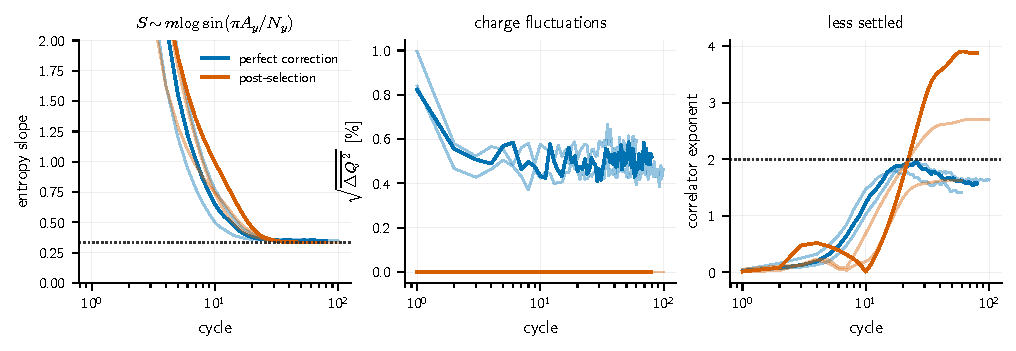
\includegraphics[width=\columnwidth]{figures/init_default_scaling.pdf}
  \caption{Init-default streaming diagnostics.  Entanglement slopes flow toward the
  chiral value $1/3$, while the charge-sector RMS separates the physical stochastic
  perfect-correction ensemble from the post-selected branch.  Correlator exponents are
  shown as a warning: their finite-size and protocol dependence is stronger than the
  entropy-slope evidence.}
  \label{fig:init_default}
\end{figure}

The key interpretation is not that post-selection and perfect correction are numerically
identical.  Rather, the entropy slope is a robust chiral-critical diagnostic, while the
charge-sector statistics remember whether measurement randomness was sampled or removed.
The perfect-correction ensemble is therefore the object relevant to physical adaptive
preparation.

\section{Max-mix purification}

The max-mix purification campaigns provide a complementary view.  Starting from a highly
mixed covariance, the adaptive protocol purifies toward a topological domain-wall ensemble.
Figure~\ref{fig:purification} shows that perfect correction drives the residual entropy
well below the post-selected value, while preserving small but nonzero charge fluctuations.
Post-selection gives a cleaner Chern marker and a characteristic residual entropy near
$2\log 2$, but it does so by following the conditioned branch.

\begin{figure}[t]
  \centering
  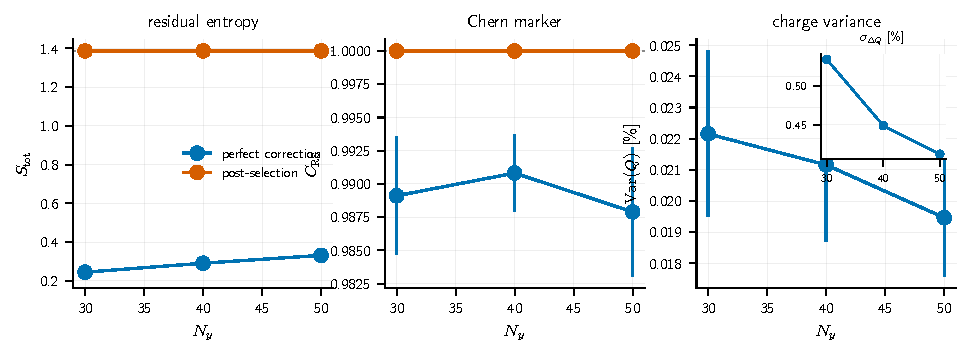
\includegraphics[width=\columnwidth]{figures/purification_protocol_comparison.pdf}
  \caption{Max-mix purification at final cycle for the $N_x=20$ campaign.  Perfect
  correction and post-selection both recover the topological marker, but they differ
  strongly in residual entropy and charge fluctuations.  The dotted entropy line marks
  $2\log 2$.}
  \label{fig:purification}
\end{figure}

This distinction is precisely the desired phenomenology.  The protocol is not merely
projecting onto a fixed charge sector.  Under perfect correction the measurement record
remains random and generates a charge-fluctuating ensemble of chiral critical states.

\section{Trajectory-resolved observables versus the mean channel}

The sharpest mathematical point is the noncommutativity of nonlinear observables with
trajectory averaging.  For a linear one-body observable $A$,
\begin{equation}
  \avg{\Tr(A C_\xi)} = \Tr(A\bar C).
\end{equation}
For entropy and squared correlations this simplification fails.  For example,
\begin{equation}
  \avg{|C_\xi(r,r')|^2}
  =
  |\bar C(r,r')|^2
  +
  \avg{|C_\xi(r,r')-\bar C(r,r')|^2}.
  \label{eq:square_corr_decomp}
\end{equation}
The second term is exactly the trajectory-to-trajectory fluctuation contribution.  Removing
it by studying only $|\bar C|^2$ changes the long-distance diagnostic.

\begin{figure}[t]
  \centering
  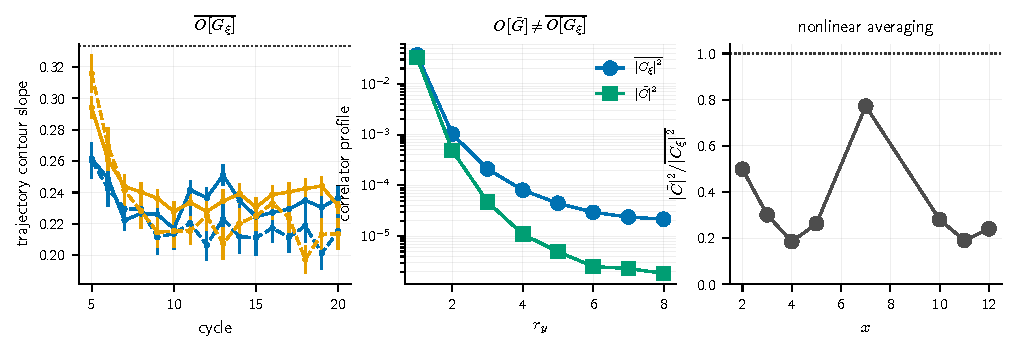
\includegraphics[width=\columnwidth]{figures/trajectory_vs_mean_channel.pdf}
  \caption{Trajectory-resolved adaptive diagnostics compared with mean-covariance controls.
  Left: trajectory-resolved contour-slope statistics from sampled perfect-correction
  histories.  Center and right: existing correlation-profile data showing
  $\overline{|C_\xi|^2}$ differs systematically from $|\bar C|^2$.}
  \label{fig:mean_channel}
\end{figure}

The Lindblad approximation inherits this status.  It is a continuous-time description of
the mean channel, not of the full stochastic ensemble.  It is therefore appropriate for
explaining averaged covariance convergence, but not for replacing the trajectory-resolved
critical-state diagnostics.

\section{Entanglement and correlation scaling}

Figure~\ref{fig:critical_scaling} collects the main scaling evidence.  The large-$N_y$
entanglement fits approach slopes in the vicinity of $1/3$ with high linear-fit quality.
Across $N_y=30,40,50$ final-cycle runs the slopes sit slightly above the ideal value,
consistent with finite-size corrections and finite circuit depth.  The squared-correlation
fits are qualitatively compatible with Eq.~\eqref{eq:corr_target}, but are less settled:
fixed-$x$ fits are strongly wall-position dependent, while $x$-averaged fits are closer
to the expected exponent.

\begin{figure}[t]
  \centering
  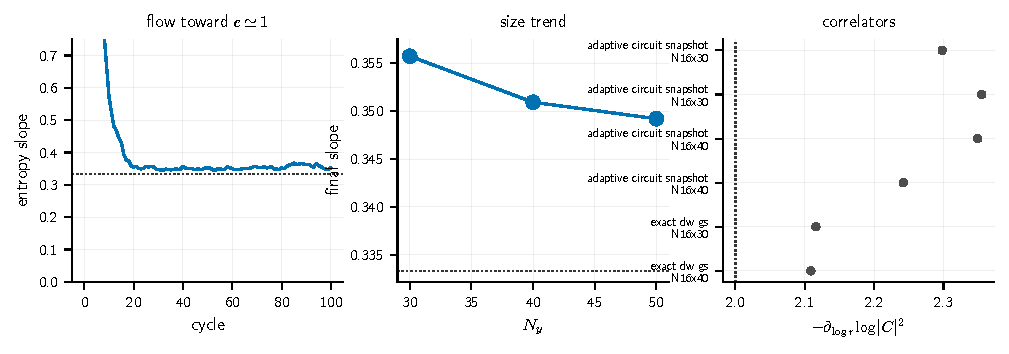
\includegraphics[width=\columnwidth]{figures/critical_scaling_summary.pdf}
  \caption{Critical-scaling summary.  Entanglement slopes approach the chiral-fermion
  target more cleanly than the currently available squared-correlation exponents.  The
  correlator panel should be read as evidence for consistency with chiral scaling, not
  as a final universality extraction.}
  \label{fig:critical_scaling}
\end{figure}

At the present stage the responsible claim is therefore asymmetric.  The entanglement
data strongly support a quasi-one-dimensional chiral critical ensemble.  The correlation
data support the same picture but require more careful finite-size, wall-window, and
trajectory-ordering analysis before being used as a precision exponent measurement.

\section{Modular charge spreading and chirality}

The modular-charge spreading diagnostics probe the orientation of the interface dynamics.
The construction inserts a localized modular charge packet and tracks its center of mass
under the modular Hamiltonian generated by the covariance.  The relevant signatures are
the signed displacement
\begin{equation}
  \Delta y_{\rm COM}(t)
  =
  y_{\rm COM}(t)-y_{\rm COM}(0),
\end{equation}
and the fitted velocity $v_y$ over a specified time window.

\begin{figure}[t]
  \centering
  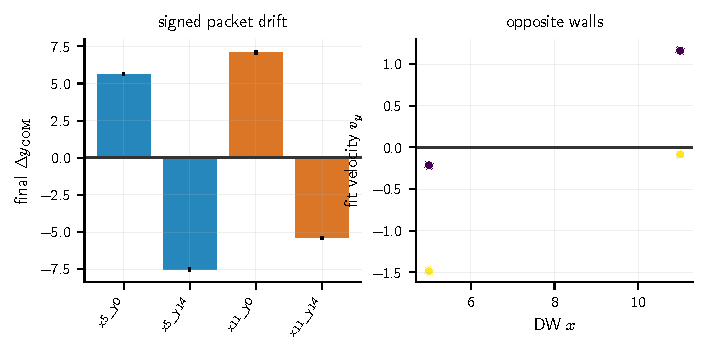
\includegraphics[width=\columnwidth]{figures/modular_charge_chirality.pdf}
  \caption{Modular-charge spreading.  Packets launched on opposite domain walls acquire
  opposite signed drift, and fitted velocities change sign between the walls.  This is
  the most direct current evidence that the domain-wall sector is chiral rather than merely
  localized.}
  \label{fig:chirality}
\end{figure}

Figure~\ref{fig:chirality} shows the essential result: packets on opposite walls drift in
opposite directions, as expected for a pair of counter-propagating chiral interfaces on a
periodic strip.  Charge conservation diagnostics in the saved summaries are at numerical
precision, so the observed motion is not a charge-leakage artifact.

\section{Hard-wall interpretation of \texorpdfstring{$dw\_truncation$}{dw truncation}}

The flattened-Hamiltonian $\alpha_2$ sweep clarifies how to interpret the production choice
\texttt{dw\_truncation=True}.  Unless otherwise stated, the production GPU scaling data use
$\alpha_1=1$ in the topological slab, a large trivial exterior mass $\alpha_2=30$,
$n_{\rm shell}=1$, and \texttt{dw\_truncation=True}.  In the model, $\alpha_1$ controls the
topological slab and $\alpha_2$ controls the exterior.  Taking $\alpha_2$ large makes the
exterior an inert trivial region.  The truncation operation enforces the corresponding
support constraint directly at the overcomplete-Wannier projector level: after the finite
shell cutoff, each mode is masked to the domain-wall region containing its center and then
renormalized.

\begin{figure}[t]
  \centering
  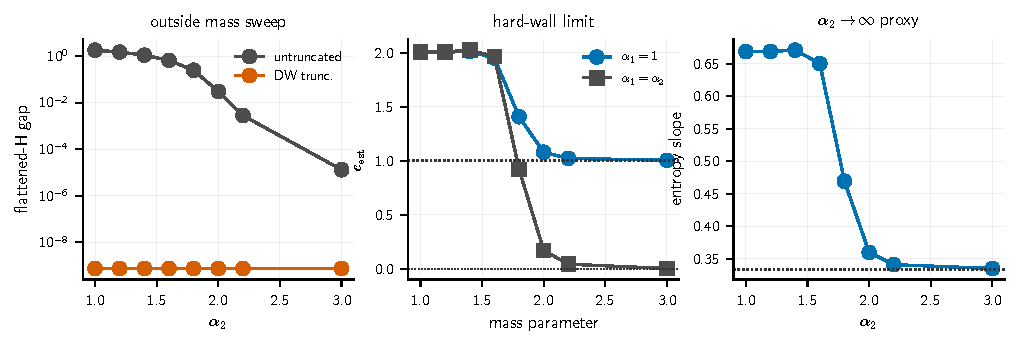
\includegraphics[width=\columnwidth]{figures/alpha2_truncation_limit.pdf}
  \caption{Flattened-Hamiltonian $\alpha_2$ sweep.  With a topological interior
  $\alpha_1=1$, increasing exterior mass under domain-wall truncation flows toward
  $c_{\rm est}\simeq 1$ and entropy slope $1/3$.  Uniform-mass truncation alone instead
  collapses toward $c\simeq0$ at large mass.  Thus truncation is an infinite-mass exterior
  approximation, not a stand-alone source of chirality.}
  \label{fig:alpha2}
\end{figure}

The correct statement is therefore not that
\begin{equation}
  \texttt{dw\_truncation} \equiv \alpha_2=\infty
\end{equation}
as a literal equality of finite Hamiltonians.  Rather, \texttt{dw\_truncation} implements
the hard-wall projector-support limit of an infinite-mass trivial exterior.  This distinction
matters because uniform-mass truncation by itself does not generate the desired large-mass
chiral state; one needs a topological interior adjacent to an inert exterior.  The
$\alpha_2$ sweep should therefore be read as a diagnostic proxy for the hard-wall limit, not
as a fully controlled extrapolation without further finite-size and truncation checks.

\section{Literature position}

The broad monitored-circuit context is the measurement-induced entanglement transition
literature \cite{LiChenFisher2018,SkinnerRuhmanNahum2019}.  For monitored free fermions,
there is now a substantial field-theoretic literature on replica/Keldysh and nonlinear-sigma
model descriptions \cite{AlbertonBuchholdDiehl2021,BuchholdMinoguchiAltlandDiehl2021,
FavaPiroliSwannBernardNahum2023,PoboikoPikulinIppoliti2023,StarchlFischerSieberer2025}.
Those works are essential background for measurement-induced criticality, but the present
question is different: the monitored degrees of freedom are class-A Chern-band projectors,
and the critical sector is tied to a domain-wall chiral edge rather than to a one-dimensional
bulk monitoring transition.

The distinction between physical Born-rule trajectories and forced or post-selected ensembles
is also not optional.  Different trajectory ensembles can have different replica limits and
different universal behavior \cite{JianShapourianBauerLudwig2023,LeungMeidanRomito2025,
LeGalTurkeshiSchiro2023}.  This is the conceptual reason that post-selection is treated
here as a control, not as the physical adaptive preparation.

The dissipative-control context is the Lindblad preparation of Chern insulators
\cite{DiehlRicoBaranovZoller2011,BudichZollerDiehl2015,Goldstein2019} and the topology of
Gaussian mixed states \cite{BudichDiehl2015,BardynWawerAltlandFleischhauerDiehl2018,
WawerFleischhauer2021}.  Those works are closest to the mean-channel and Lindblad-limit
controls, not to the full trajectory-resolved perfect-correction ensemble.  The monitored
topological-dynamics setting is closer to the transfer-matrix and adaptive-circuit programs
\cite{JianBauerKeselmanLudwig2022,PanShapourianJian2025,BhuiyanPanJian2026}, with the
present note zooming in on the chiral domain-wall sector.

Finally, the modular-charge results are naturally compared with chiral modes and transport
along Chern-insulator or quantum-anomalous-Hall domain walls
\cite{CallanHarvey1985,Hatsugai1993,QiWuZhang2006,UpadhyayaTserkovnyak2016,RosenEtAl2017},
while remaining a covariance/modular-flow diagnostic rather than a transport measurement in
a material.

\section{Open numerical issues}

Several points should be settled before this becomes a final manuscript.
First, the correlator exponent extraction needs a controlled comparison of fixed-wall,
wall-window, and full-$x$ averaged observables, with the ensemble ordering fixed throughout.
Second, the Markov-channel and Lindblad controls should be used to explain which features
survive covariance averaging and which are specifically trajectory-resolved.  Third, the
modular-charge chirality evidence should be extended to more sizes and launch windows.
Fourth, the $\alpha_2$ sweep should be exported into a stable table rather than remaining
encoded in notebook outputs.  None of these caveats undercuts the main story, but they
determine what can be claimed quantitatively.

\section{Conclusion}

The coherent story is now clear.  The finite-range class-A adaptive circuit does more than
prepare a bulk Chern marker.  Under trajectory-resolved perfect correction it prepares an
ensemble whose domain-wall sector has logarithmic entanglement scaling, charge-sector
fluctuations, and chiral modular-charge spreading.  Post-selection, the Markov channel, and
the Lindblad limit are indispensable controls precisely because they remove or average the
measurement-record randomness in different ways.  The physical phenomenon is the stochastic
adaptive ensemble itself:
\[
  \boxed{
  \avg{O[\Gtraj]}
  \;\hbox{is the object prepared by perfect correction.}
  }
\]
It is neither the mean-channel observable $O[\Gbar]$ nor the post-selected observable
$O[\Gps]$.

\begin{acknowledgments}
This note was generated as a repository-level synthesis of existing data products, figures,
and notebooks in \texttt{class\_A\_fermionic\_adaptive\_circuit}.  It excludes
\texttt{erroneous\_gpu\_stuff}.
\end{acknowledgments}

\begin{thebibliography}{99}

\bibitem{BhuiyanPanJian2026}
A.~Bhuiyan, H.~Pan, and C.-M.~Jian,
``Free-fermion dynamics with measurements: Topological classification and adaptive preparation of topological states,''
Phys. Rev. Research \textbf{00}, 003000 (2026).

\bibitem{LiChenFisher2018}
Y.~Li, X.~Chen, and M.~P.~A. Fisher,
``Quantum Zeno effect and the many-body entanglement transition,''
Phys. Rev. B \textbf{98}, 205136 (2018).

\bibitem{SkinnerRuhmanNahum2019}
B.~Skinner, J.~Ruhman, and A.~Nahum,
``Measurement-induced phase transitions in the dynamics of entanglement,''
Phys. Rev. X \textbf{9}, 031009 (2019).

\bibitem{AlbertonBuchholdDiehl2021}
O.~Alberton, M.~Buchhold, and S.~Diehl,
``Entanglement transition in a monitored free-fermion chain: From extended criticality to area law,''
Phys. Rev. Lett. \textbf{126}, 170602 (2021).

\bibitem{BuchholdMinoguchiAltlandDiehl2021}
M.~Buchhold, Y.~Minoguchi, A.~Altland, and S.~Diehl,
``Effective theory for the measurement-induced phase transition of Dirac fermions,''
Phys. Rev. X \textbf{11}, 041004 (2021).

\bibitem{FavaPiroliSwannBernardNahum2023}
M.~Fava, L.~Piroli, T.~Swann, D.~Bernard, and A.~Nahum,
``Nonlinear sigma models for monitored dynamics of free fermions,''
Phys. Rev. X \textbf{13}, 041045 (2023).

\bibitem{PoboikoPikulinIppoliti2023}
I.~Poboiko, D.~I. Pikulin, and M.~Ippoliti,
``Measurement-induced phase transition for free fermions above one dimension,''
Phys. Rev. X \textbf{13}, 041046 (2023).

\bibitem{StarchlFischerSieberer2025}
E.~Starchl, L.~E. Fischer, and L.~M. Sieberer,
``Generalized Zeno effect and entanglement dynamics in monitored free fermions,''
arXiv:2406.07673.

\bibitem{JianShapourianBauerLudwig2023}
C.-M. Jian, H.~Shapourian, B.~Bauer, and A.~W. W. Ludwig,
``Measurement-induced criticality in random quantum circuits,''
arXiv:2302.09094.

\bibitem{LeungMeidanRomito2025}
C.~Y. Leung, D.~Meidan, and A.~Romito,
``Measurement-induced transitions in free fermions with partial postselection,''
Phys. Rev. X \textbf{15}, 021020 (2025).

\bibitem{LeGalTurkeshiSchiro2023}
Y.~Le Gal, X.~Turkeshi, and M.~Schiro,
``Volume-to-area-law entanglement transition in a non-Hermitian free fermionic chain,''
SciPost Phys. \textbf{14}, 138 (2023).

\bibitem{DiehlRicoBaranovZoller2011}
S.~Diehl, E.~Rico, M.~A. Baranov, and P.~Zoller,
``Topology by dissipation in atomic quantum wires,''
Nat. Phys. \textbf{7}, 971 (2011).

\bibitem{BudichZollerDiehl2015}
J.~C. Budich, P.~Zoller, and S.~Diehl,
``Dissipative preparation of Chern insulators,''
Phys. Rev. A \textbf{91}, 042117 (2015).

\bibitem{Goldstein2019}
M.~Goldstein,
``Dissipation-induced topological insulators: A no-go theorem and a recipe,''
SciPost Phys. \textbf{7}, 067 (2019).

\bibitem{BudichDiehl2015}
J.~C. Budich and S.~Diehl,
``Topology of density matrices,''
Phys. Rev. B \textbf{91}, 165140 (2015).

\bibitem{BardynWawerAltlandFleischhauerDiehl2018}
C.-E. Bardyn, L.~Wawer, A.~Altland, M.~Fleischhauer, and S.~Diehl,
``Probing the topology of density matrices,''
Phys. Rev. X \textbf{8}, 011035 (2018).

\bibitem{WawerFleischhauer2021}
L.~Wawer and M.~Fleischhauer,
``Chern number and Berry curvature for Gaussian mixed states of fermions,''
Phys. Rev. B \textbf{104}, 094104 (2021).

\bibitem{JianBauerKeselmanLudwig2022}
C.-M. Jian, B.~Bauer, A.~Keselman, and A.~W. W. Ludwig,
``Criticality and entanglement in nonunitary quantum circuits and tensor networks of noninteracting fermions,''
Phys. Rev. B \textbf{106}, 134206 (2022).

\bibitem{PanShapourianJian2025}
H.~Pan, H.~Shapourian, and C.-M. Jian,
``Topological modes and domain walls in monitored free-fermion dynamics,''
Phys. Rev. B \textbf{112}, 144301 (2025).

\bibitem{CallanHarvey1985}
C.~G. Callan and J.~A. Harvey,
``Anomalies and fermion zero modes on strings and domain walls,''
Nucl. Phys. B \textbf{250}, 427 (1985).

\bibitem{Hatsugai1993}
Y.~Hatsugai,
``Chern number and edge states in the integer quantum Hall effect,''
Phys. Rev. Lett. \textbf{71}, 3697 (1993).

\bibitem{QiWuZhang2006}
X.-L. Qi, Y.-S. Wu, and S.-C. Zhang,
``Topological quantization of the spin Hall effect in two-dimensional paramagnetic semiconductors,''
Phys. Rev. B \textbf{74}, 085308 (2006).

\bibitem{UpadhyayaTserkovnyak2016}
P.~Upadhyaya and Y.~Tserkovnyak,
``Domain wall in a quantum anomalous Hall insulator as a magnetoelectric piston,''
Phys. Rev. B \textbf{94}, 020411(R) (2016).

\bibitem{RosenEtAl2017}
I.~T. Rosen \textit{et al.},
``Chiral transport along magnetic domain walls in the quantum anomalous Hall effect,''
npj Quantum Mater. \textbf{2}, 69 (2017).

\end{thebibliography}

\end{document}
